\begin{figure}[h]
\begin{center}
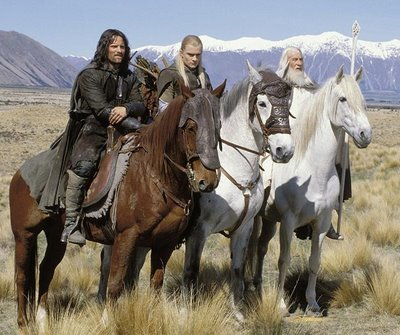
\includegraphics[width=0.6\textwidth] {imagenes/caballos.jpeg}
\end{center}
\end{figure}

\subsection{Problema a resolver}
El problema a resolver consiste en dar un algoritmo de Backtracking que minimice la cantidad de caballos utilizados para cubrir todos los casilleros de un tablero de $n$ x $n$.

Decimos que un casillero está cubierto sí está ocupado con un caballo o es amenazado por otro caballo.

A su vez, el tablero inicial puede o no tener caballos ya posicionados, en cuyo caso igual se quiere buscar la solución optima que minimice la cantidad de caballos utilizados.

\begin{itemize}
\item Ejemplo 1: Situación inicial.

\begin{codesnippet}
n = 8, sin caballos iniciales
\end{codesnippet}
\item Solución del ejemplo\footnote{Se puede encontrar las soluciones para $3 \leq n \leq 17$ con tableros vacios en \url{http://home.earthlink.net/~morgenstern/solution/knsols1.htm}}:

\begin{codesnippet}
Cantidad de caballos agregados: 12
Tablero:
0 0 0 0 0 0 0 0
0 0 1 0 0 0 0 0
0 0 1 1 0 1 1 0
0 0 0 0 0 1 0 0
0 0 1 0 0 0 0 0
0 1 1 0 1 1 0 0
0 0 0 0 0 1 0 0
0 0 0 0 0 0 0 0
\end{codesnippet}
\end{itemize}

\subsection{Resolución planteada}
La solución planteada utiliza la técnica algorítmica de backtracking, como se pide en el enunciado. La idea es recorrer el tablero inicial evaluando cada posición vacía (es decir sin caballo. Puede ser vacía y estar amenazada) para determinar si es necesario poner un caballo o, en caso contrario, comparar las mejores soluciones al poner un caballo en la casilla o dejarla como estaba.

Nuestro modelo consiste en representar el tablero con una matriz de tamaño $n*n$. De esta manera conseguimos acceder a cada dato del tablero en tiempo constante. Dicho esto, nuestro algoritmo va 'procesando' cada casilla sin caballo secuencialmente de izquierda a derecha y de arriba hacia abajo. Es decir que empieza desde la primer casilla sin un caballo (x,y), toma las decisiones correspondientes a la casilla, se fija si la casilla (x,y+1) tiene un caballo, si no lo tiene la 'procesa', en caso contrario se fija la casilla (x, y+2), (x, y+3), ... , (x, n-1) , (x+1, 0) , ... , (x+1, n-1) , (n-1, 0) y asi hasta (n-1, n-1).

Para ayudar a tomar estas decisiones hemos pensado e implementado una serie de \textit{podas} que evitan llegar a soluciones invalidas o (parcialmente) suboptimas. Consideramos que se va a llegar a una solución invalida cuando, al visitar una casilla sin caballo que no esta amenazada, no ponerle un caballo implica que no pueda ser amenazada en el futuro. Es decir que no hay habría manera de colocar un caballo en una casilla a ser visitada en el futuro de manera que aquella casilla quede amenazada. De esto se encargan las podas 'B' y 'C', las cuales explicamos en la próxima sección. Las demás podas se encargan de no considerar decisiones que necesariamente llevarían a soluciones subóptimas (tableros en los cuales todas las casillas tienen un caballo o están amenazadas, pero cuya cantidad de caballos es mayor a la de otra solución).


\subsubsection{Poda A}
Este caso se da cuando todas las posiciones que amenaza el casillero siendo evaluado tienen un caballo o están amenazadas y alguna al menos tiene un caballo, es decir, la casilla actual esta amenazada.
Si pasa esto, entonces el casillero siendo evaluado tiene que permanecer vacío. Porque si pusiera un caballo, entonces me llevaría a una solución sub-optima, ya que estaría poniendo un caballo que no es realmente necesario.

\begin{itemize}
\item Notación: 'c' es el casillero siendo evaluado, 'a' son las posiciones amenazadas, '1' son las casillas que tienen un caballo.

\item Ejemplo: Situación inicial.

\begin{codesnippet}
Tablero (c es el casillero siendo evaluado):
c 0 a 0
0 0 a 0
0 1 0 0
0 0 0 1
\end{codesnippet}

\item Decisión subóptima:

\begin{codesnippet}
Tablero:
1 0 a 0
0 0 a 0
0 1 0 0
0 0 0 1
\end{codesnippet}

\item Decisión óptima:

\begin{codesnippet}
Tablero:
a 0 a 0
0 0 a 0
0 1 0 0
0 0 0 1
\end{codesnippet}
\end{itemize}

\subsubsection{Poda B}
Este caso se da cuando existe una posición que amenaza el casillero siendo evaluado que ya fue procesada, está vacía y solo la puede amenazar el casillero siendo evaluado (todas las otras posiciones que pueden amenazar a la amenazada ya fueron procesadas y ninguna tiene un caballo).
Si pasa esto, entonces el casillero siendo evaluado tiene que tener un caballo sí o sí. Dejarlo vacío me llevaría a una tablero incorrecto, porque sería imposible amenazar el otro casillero en el futuro.

\begin{itemize}
\item Ejemplo: Situación inicial.

\begin{codesnippet}
Tablero (c es el casillero siendo evaluado):
0 0 0 0
0 0 a 0
0 c 0 0
0 0 0 1
\end{codesnippet}

\item Decisión incorrecta:
en este caso, amenazar la casilla (0,0) se vuelve imposible

\begin{codesnippet}
Tablero:
0 0 0 0
0 0 a 0
0 a c 0
0 0 0 1
\end{codesnippet}

\item Decisión correcta:

\begin{codesnippet}
Tablero:
a 0 a 0
0 0 a a
0 1 c 0
0 0 0 1
\end{codesnippet}
\end{itemize}

\subsubsection{Poda C}
Este caso se da cuando todas las posiciones que amenaza el casillero siendo evaluado ya fueron procesadas y ninguna tiene un caballo.
Si pasa esto, entonces el casillero siendo evaluado tiene que tener un caballo sí o sí. Porque si se lo deja vacío, no hay forma de amenazarlo en el futuro.

\begin{itemize}
\item Ejemplo: Situación inicial.

\begin{codesnippet}
Tablero (c es el casillero siendo evaluado):
1 1 1
a c a
a a a
\end{codesnippet}

\item Decisión incorrecta:

\begin{codesnippet}
Tablero:
1 1 1
a 0 a
a a a
\end{codesnippet}

\item Decisión correcta:

\begin{codesnippet}
Tablero:
1 1 1
a 1 a
a a a
\end{codesnippet}
\end{itemize}

\subsubsection{Poda D}
Este caso se da cuando existe una posición que el casillero siendo evaluado amenaza que tiene un caballo, y a la vez, todas sus posiciones amenazadas que no son la actual tienen caballo. Además, no se deben cumplir \textit{B} o \textit{C}.
Si pasa esto, entonces el casillero siendo evaluado tiene que permanecer vacío, excepto que el caballo amenazado halla sido puesto a través del input. En caso contrario, si pusiera un caballo me llevaría a una solución sub-optima, porque el casillero amenazado, estaría siendo amenazado por todas las posiciones posibles y además tendría un caballo. Casos en los que una posición contiene un caballo y, a la vez, todas sus posiciones amenazadas contienen un caballo llevan a tableros subóptimos, porque poner un caballo allí no cambia el total de casillas amenazadas.

\begin{itemize}
\item Ejemplo: Situación inicial.

\begin{codesnippet}
Tablero (c es el casillero siendo evaluado):
c a 0 0
a 0 1 0
1 a a a
0 1 a 1
\end{codesnippet}

\item Solución parcial subóptima:

\begin{codesnippet}
Tablero:
1 a 0 0
a 0 1 0
1 a a a
0 1 a 1
\end{codesnippet}

\item Solución parcial óptima:

\begin{codesnippet}
Tablero:
a a 0 0
a 0 1 0
1 a a a
0 1 a 1
\end{codesnippet}
\end{itemize}

\subsubsection{Poda G}
Esta poda consiste en calcular una cota como primer aproximación a la cantidad de caballos necesarios para la solución óptima usando un \textit{algoritmo goloso}. Si en algún paso del algoritmo del ejercicio la cantidad de caballos supera esta cota, dejamos de calcular dicha solución, porque la solución que nos dio el algoritmo goloso es mejor (esto lo generaliza la poda Z).

La cota en cuestión se calcula antes de empezar el algoritmo de backtracking.

El algoritmo goloso que se utiliza para esta cota buscará en cada paso maximizar la cantidad de posiciones amenazadas al poner un caballo. Es decir, compara la cantidad de nuevas casillas amenazadas entre varios casilleros y se queda con la mejor, y asi recorre cada casilla del tablero una sola vez.

Como claramente este problema no adhiere al \textit{principio de optimalidad}, la solución dada no será óptima en principio, pero en general es una aproximación más interesante que usar como cota $n^2$.

\subsubsection{Poda S}
Esta poda funciona de manera muy parecida a lo que hace la \textit{Poda G}. Sin embargo, en este caso la cota a utilizar es la cantidad de caballos en la mejor solución que se conoce para un Tablero de ese tamaño (o sea, para un $n$ dado). Esta información fue recompilada del sitio mencionado en la sección de \textit{Problema a resolver} y tiene dichos valores para $3\leq n\leq 17$.

De esta forma, sí en algún momento encontramos una solución con cantidad de caballos igual a la cantidad de caballos utilizada en la solución optima, sabemos que no tenemos que seguir buscando y ya podemos dar la solución.

Es necesario notar, que los valores recompilados solo sirven para soluciones en las que el Tablero inicial esté vacío. Es por eso que esta poda además tiene en cuenta la cantidad de caballos iniciales. Sí en algún momento la solución parcial actual tiene más caballos que la solución optima más los caballos iniciales, entonces sabemos que podemos podar dicha solución, ya que no será optima.

\subsubsection{Poda Z}
Esta poda funciona de manera muy parecida a lo que hace la \textit{Poda G}. Sin embargo, en este caso la cota a utilizar es la cantidad de caballos en la mejor solución encontrada hasta el momento. De esta forma, una vez que nuestro algoritmo encuentre una solución de $k$ caballos, automaticamente empezara a podar todos los subarboles que tengan soluciones parciales con $k+1$ caballos.

\subsubsection{Pseudocódigo}
Para hacer el pseudocódigo más sencillo, no vamos a listar las condiciones que tienen que pasar para cada Poda, ya que cada una fue explicada más arriba con ejemplos.

\begin{codesnippet}
main:
	pongo tablero_inicial = un tablero vacio más los caballos pasados por input
	pongo cota_optima = resolver_con_goloso(tablero_inicial)
	result = resolver_aux(cota_optima, (0,0))

resolver_aux(optimo_alcanzado, ultima_celda):
	Si entro en los casos de las podas G, S o Z
		devuelvo la cantidad de caballos utilizados por la solución optima \
			alcanzada
	pongo siguiente = siguiente celda vacía sin un caballo en el tablero \
		después de ultima_celda
	Si no hay siguiente
		devuelvo el mínimo entre la cantidad de caballos usada por la \ 
			solución actual y la solución optima alcanzada
    Si entro en el caso de la poda A
		dejo la celda como esta y llamo a resolver_aux recursivamente
	Si entro en el caso de la poda B
		pongo un caballo en la celda y llamo a resolver_aux recursivamente
	Si entro en el caso de la poda C
		dejo la celda como esta y llamo a resolver_aux recursivamente
	Si entro en el caso de la poda D (y no entre en los casos B ni C)
		pongo un caballo en la celda y llamo a resolver_aux recursivamente
	Si no entre a ningún caso de poda
		pruebo llamando a resolver_aux recursivamente: dejando vacío y \
			poniendo un caballo en la celda
		devuelvo el mínimo de esos dos

resolver_con_goloso(tablero):
	pongo siguiente = siguiente celda vacia no amenazada en el tablero
    Si no hay siguiente
		devuelvo la cantidad de caballos usada
	pongo posibilidades = [las posibles formas de poner un caballo que haga
		que la celda "siguiente" este cubierta]
	tomo de posibilidades la que maximize la cantidad de celdas cubiertas
	agrego al tablero la decision tomada
	llamo resolver_con_goloso(tablero)

\end{codesnippet}

\subsubsection{Justificación}

Como planteamos en nuestra resolución, nuestro algoritmo primero encuentra una solución aproximada usando un algoritmo auxiliar goloso. Luego, procede visitando cada celda sin un caballo secuencialmente. Las podas desechan tableros incorrectos y decisiones que necesariamente llevarían a tableros con más caballos de lo necesario. Finalmente, si ninguna poda aplica, compara las soluciones dadas entre dejar un casillero vacío y poner un caballo en ese lugar.

\subsection{Complejidad propuesta}
Dado un Tablero de $n$ x $n$, el algoritmo propuesto evalúa cada celda de forma secuencial una sola vez, y ya que para cada celda hay dos posibilidades, o bien poner un caballo o bien dejarla vacía, el árbol de decisión tendría $2^{M}$ nodos, donde \textit{M} es la cantidad de celdas a evaluar.

Por ejemplo, en un tablero vacío de largo \textit{n}, $M= n^2$. Sin embargo, si el tablero inicial tiene k celdas con caballos ya cargados, entonces tenemos $M=n^2 - k$, pues hay $k$ celdas para las cuales no hay que decidir si tiene o no un caballo.

Ahora, para ver que el algoritmo propuesto tiene complejidad $\mathcal{O}(2^{n^2 - k})$, tenemos que ver que las operaciones realizadas en cada nodo (sin contar las llamadas recursivas y guardar un nuevo tablero, explicado a continuación) tienen costo constante. En nuestro caso, realizamos distintas comparaciones de enteros y checkeos para las podas. Estos checkeos, a su vez, consisten en recorrer las posiciones a las cuales amenazaría un caballo colocado en la posición actual. Como la cantidad de posiciones que un caballo puede amenazar es a lo sumo 8, podemos decir que este ciclo se repite una cantidad constante de veces. Dentro del ciclo, solo se realizan operaciones constantes. Por lo tanto, en cada paso, se realizan a lo sumo dos llamadas recursivas y operaciones de costo constante.

Cuando llegamos a soluciones del tablero con menos cantidad de caballos que la mejor solución calculada hasta el momento, queremos guardar el tablero para mostrar las casillas con caballo al final del algoritmo. Si bien esta operación tiene costo $n^2$, esto no sucede muy frecuentemente. Veamos lo siguiente: el tablero se guarda solo si se encuentra uno nuevo con menos cantidad de caballos que el mejor hasta ahora, pero las posibles cantidades de caballos en el tablero son de 0 a $n^2$. Por lo tanto, como tablero se guarda como máximo $n^2$ cantidad de veces y esta operación tiene un costo de $n^2$, guardar el tablero solo añade $n^4$ trabajo a todo el algoritmo (contando todo el árbol de recursión). Entonces, estos casos no le añaden complejidad al algoritmo ya que, en particular, $n^4$ esta en $\mathcal{O}(2^{n^2 - k})$.

Además, el algoritmo propuesto utiliza una función auxiliar que con un algoritmo goloso obtiene una primera cota para la solución optima. Entonces, tenemos que ver que la complejidad de esta función es a lo sumo $\mathcal{O}(2^{n^2 - k})$. Siguiendo la notación de antes, la función auxiliar tiene \textit{M} celdas a evaluar. Para cada una de ellas checkea si obtiene más celdas cubiertas amenazándola desde alguna celda vecina, o poniendo un caballo en ella, pero solo toma una decisión por cada celda y las evalúa secuencialmente. Como vimos recién, las comparaciones toman tiempo constante ya que cada celda tiene a lo sumo 8 celdas posibles que la pueden amenazar. Por lo tanto, la complejidad de esta función es $\mathcal{O}(M)$ que es estrictamente menor que $\mathcal{O}(2^{M})$.

Luego, la complejidad del algoritmo propuesto en el peor caso es:


$$\mathcal{O}(2^{n^2 - k})$$

\newpage
\subsection{Implementación en C++}
\lstinputlisting[language=C++]{codigo/ej3.cpp}

\newpage
\subsection{Experimentación computacional}

La función utilizada para llevar a cabo las mediciones fue \texttt{std::clock}.

La complejidad teórica calculada es de $\mathcal{O}(2^{n^2 - k})$.

\subsubsection{Experimentación con instancias aleatorias}
Para generar instancias aleatorias se creo un script que utiliza la función \texttt{std::rand}. Los intervalos para los parámetros fueron:
\begin{itemize}
	\item Tamaño del tablero ($n$): 3 $\leq n \leq$ 6
   	\item Cantidad de caballos iniciales ($k$): 0 $\leq k \leq n^2$
\end{itemize}

Se generaron 200 muestras para cada combinación de n y k posibles en dichos intervalos, y para cada $x=n^2-k$ se promediaron dichas muestras.
Dichas mediciones arrojaron los siguientes resultados:

\begin{figure}[H]
        \centering
        \begin{subfigure}[b]{0.5\textwidth}
                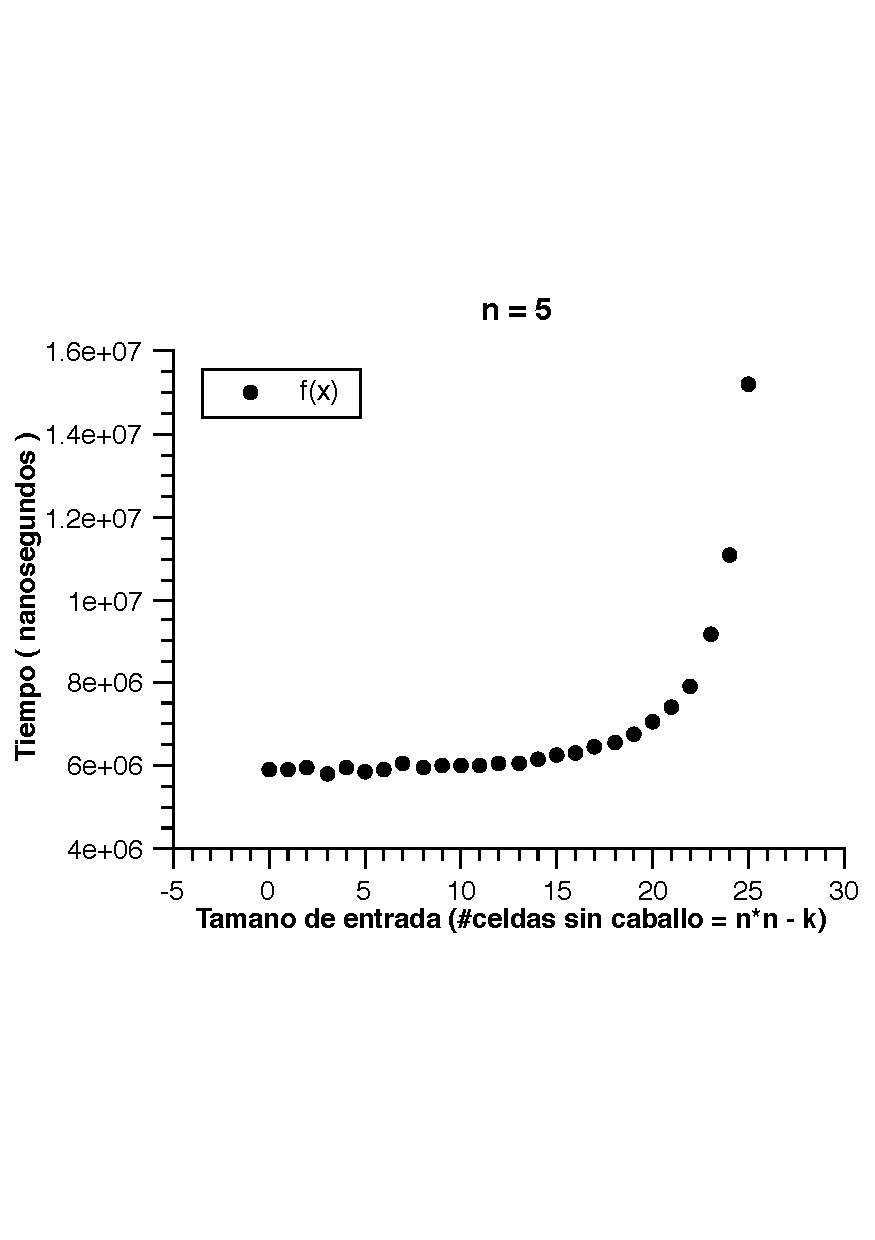
\includegraphics[width=\textwidth]{imagenes/grafico3-n-5-norm.pdf}
                \caption{Tiempos sin procesar}
        \end{subfigure}%
        ~ %add desired spacing between images, e. g. ~, \quad, \qquad, \hfill etc.
          %(or a blank line to force the subfigure onto a new line)
        \begin{subfigure}[b]{0.5\textwidth}
                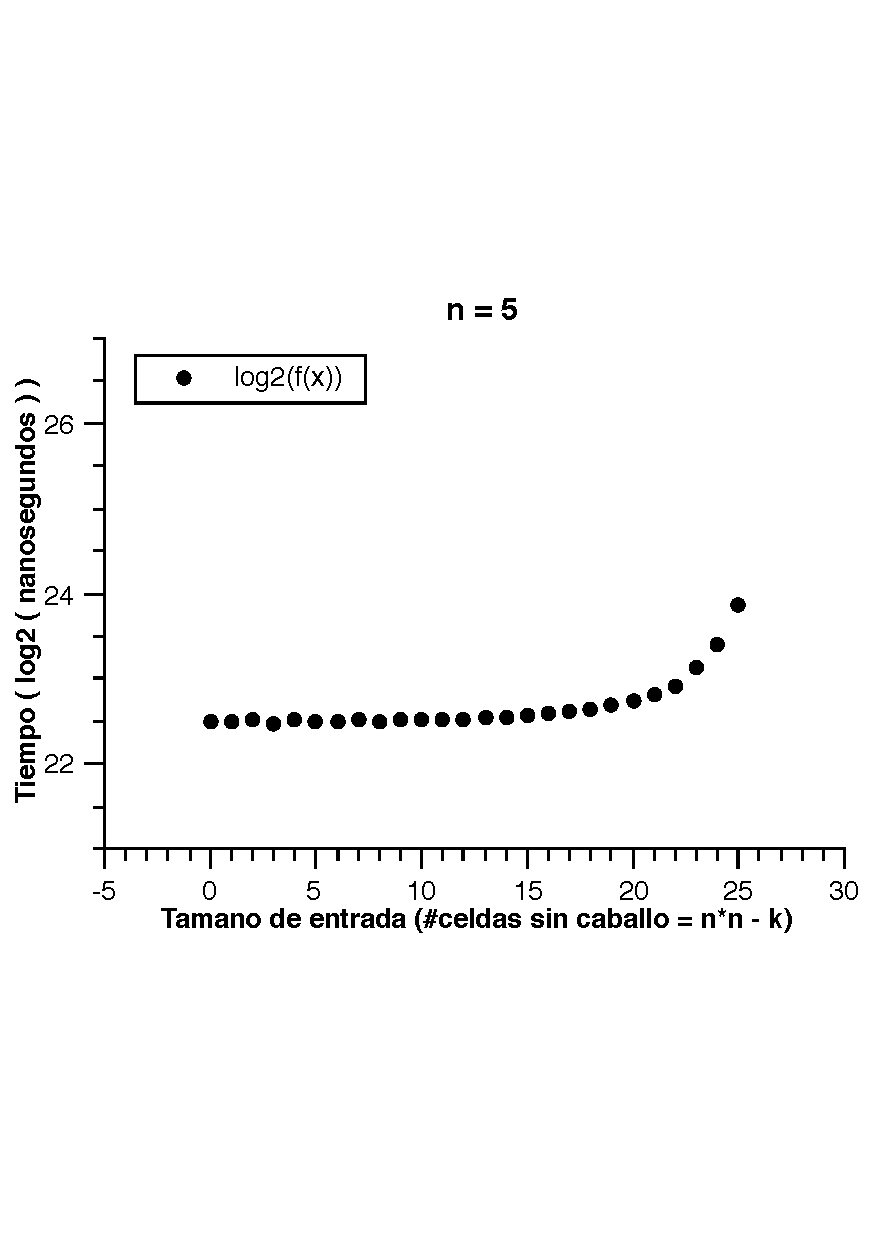
\includegraphics[width=\textwidth]{imagenes/grafico3-n-5-log.pdf}
                \caption{Logaritmo a la figura (a)}
        \end{subfigure}
        
        \begin{subfigure}[b]{0.5\textwidth}
                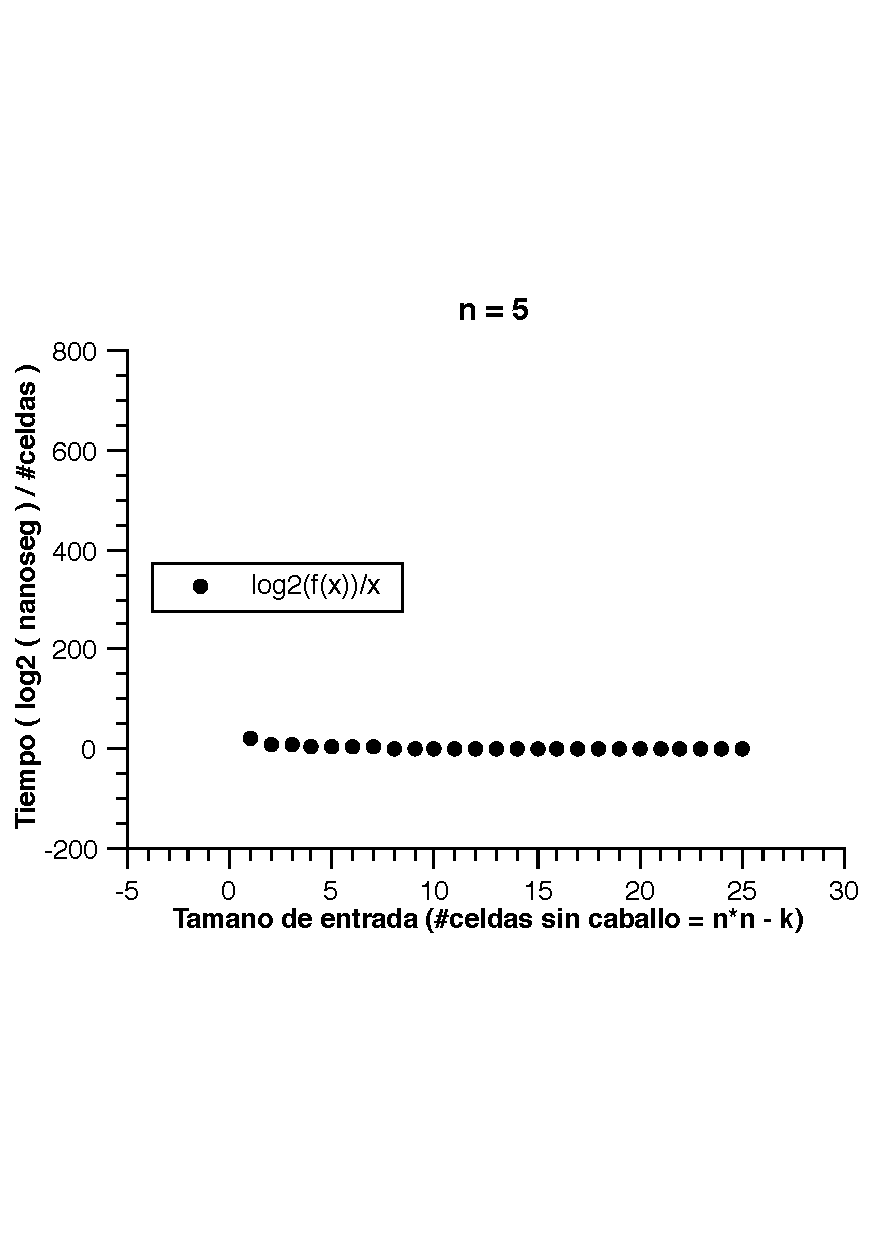
\includegraphics[width=\textwidth]{imagenes/grafico3-n-5-div-log.pdf}
                \caption{Dividiendo por x la figura (b)}
        \end{subfigure}
        \caption{Gráficos para $n=5$ sin podas G ni S}
\end{figure}

\begin{figure}[H]
        \centering
        \begin{subfigure}[b]{0.5\textwidth}
                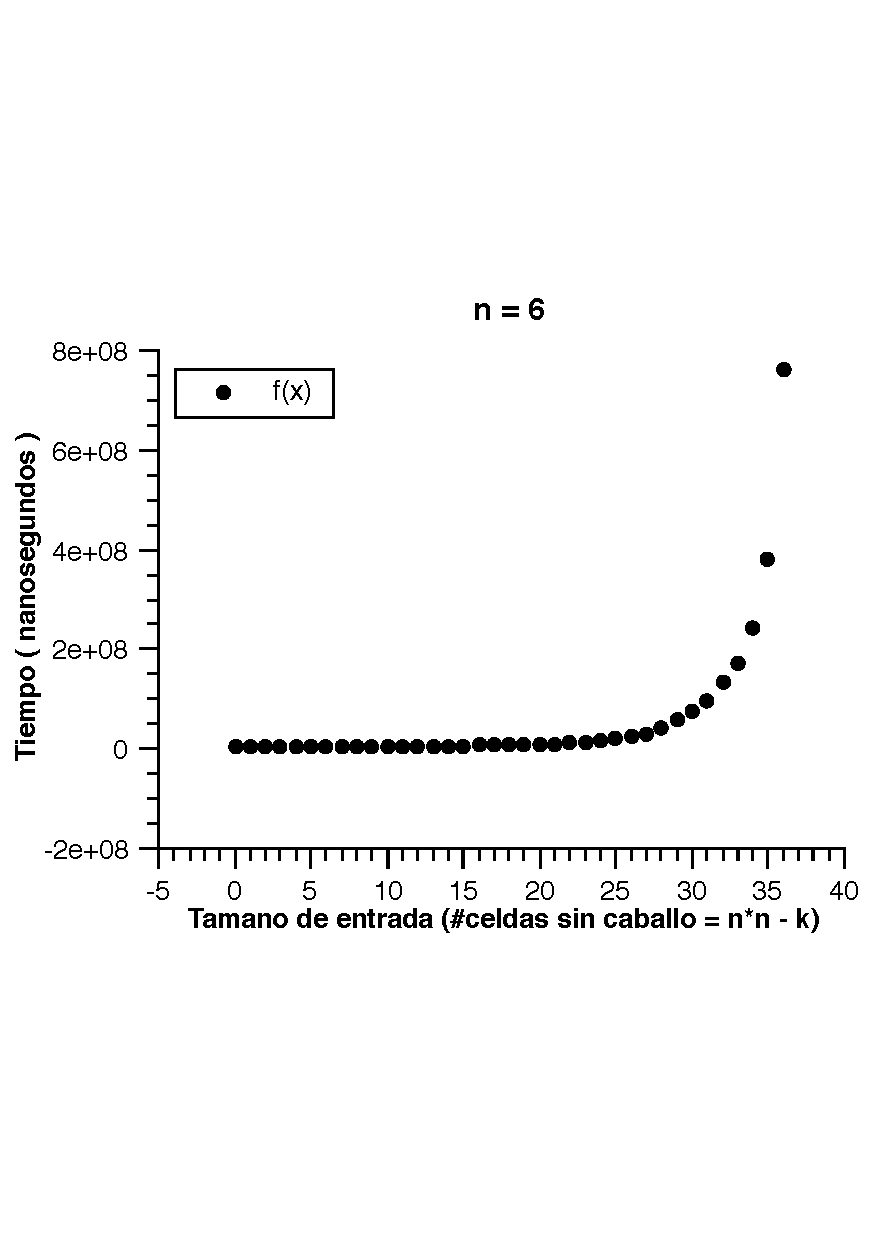
\includegraphics[width=\textwidth]{imagenes/grafico3-n-6-norm.pdf}
                \caption{Tiempos sin procesar}
        \end{subfigure}%
        ~ %add desired spacing between images, e. g. ~, \quad, \qquad, \hfill etc.
          %(or a blank line to force the subfigure onto a new line)
        \begin{subfigure}[b]{0.5\textwidth}
                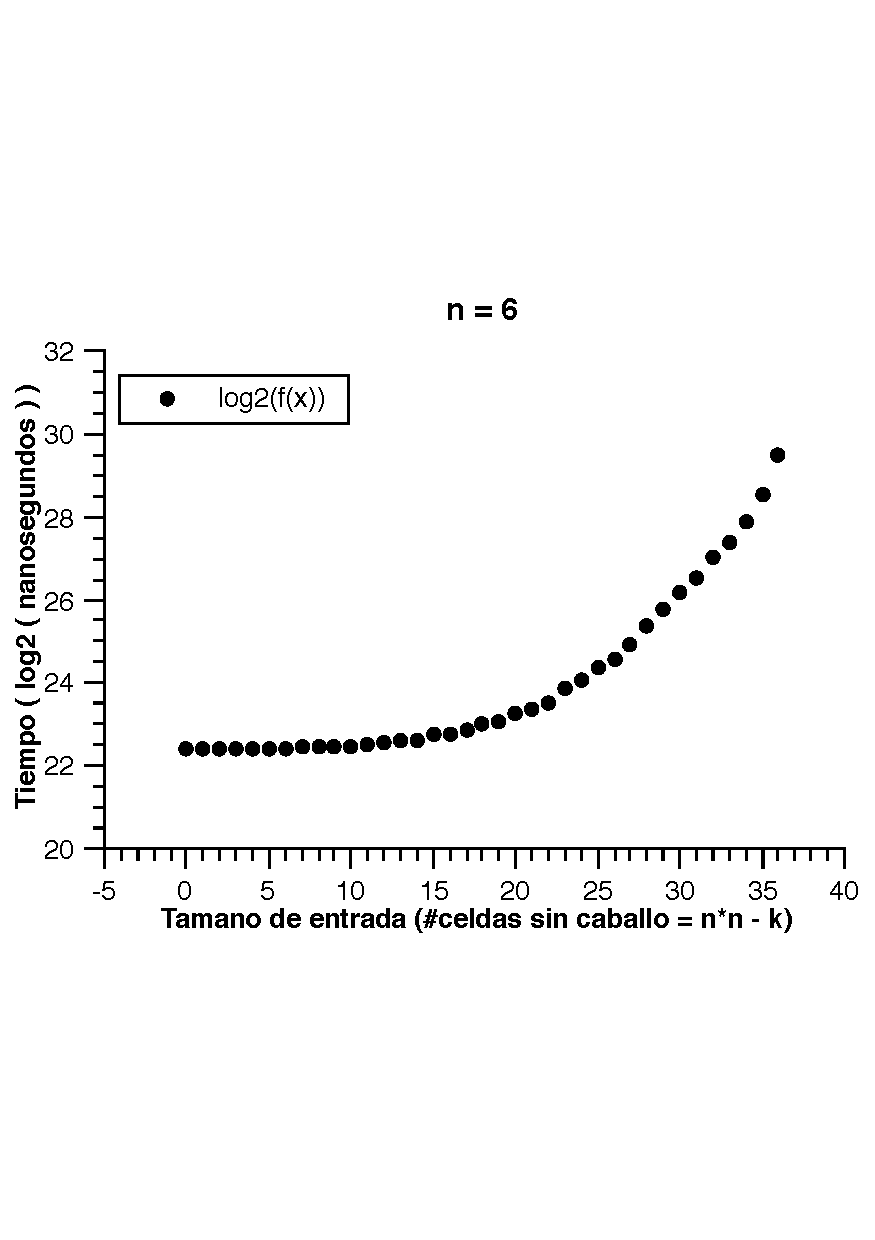
\includegraphics[width=\textwidth]{imagenes/grafico3-n-6-log.pdf}
                \caption{Logaritmo a la figura (a)}
        \end{subfigure}
        
        \begin{subfigure}[b]{0.5\textwidth}
                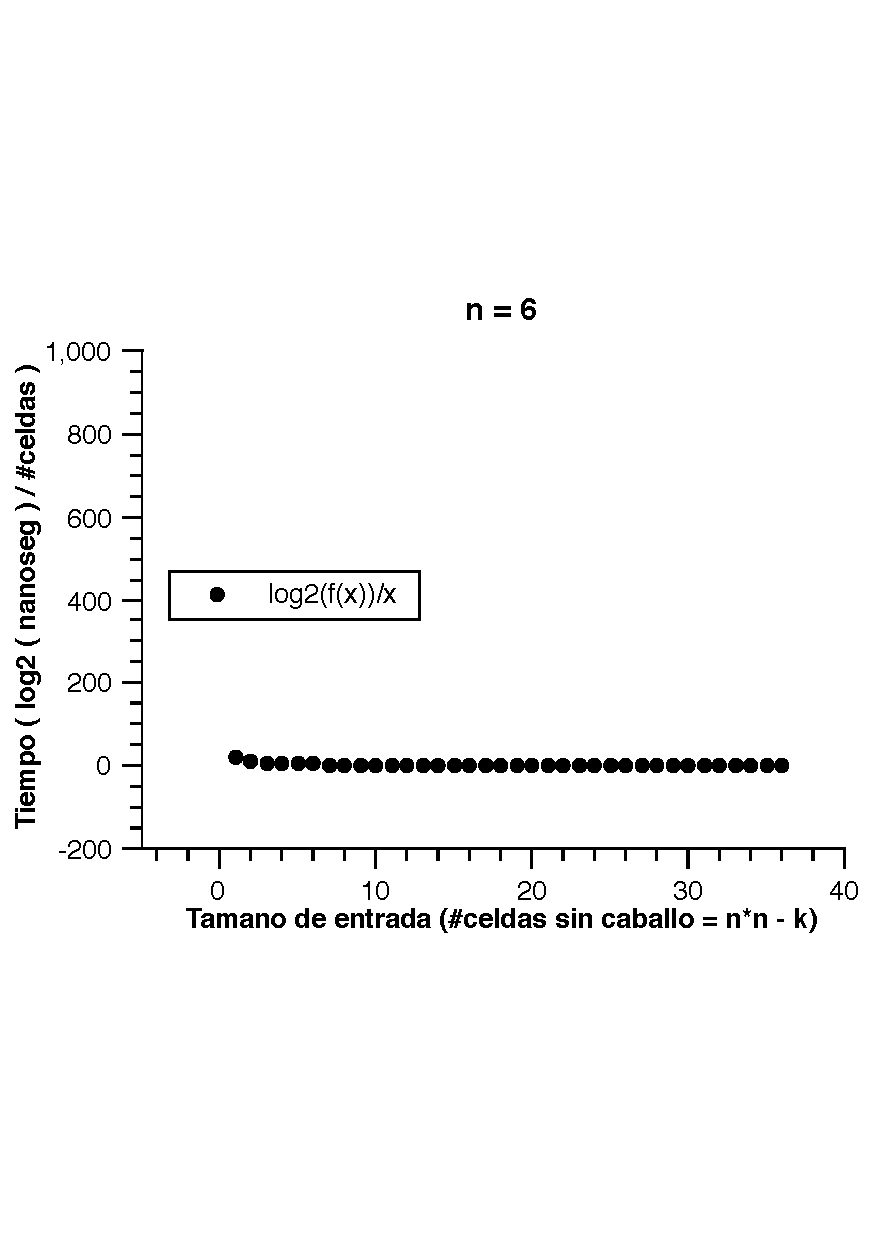
\includegraphics[width=\textwidth]{imagenes/grafico3-n-6-div-log.pdf}
                \caption{Dividiendo por x la figura (b)}
        \end{subfigure}
        \caption{Gráficos para $n=6$ sin podas G ni S}
\end{figure}

\begin{figure}[H]
        \centering
        \begin{subfigure}[b]{0.5\textwidth}
                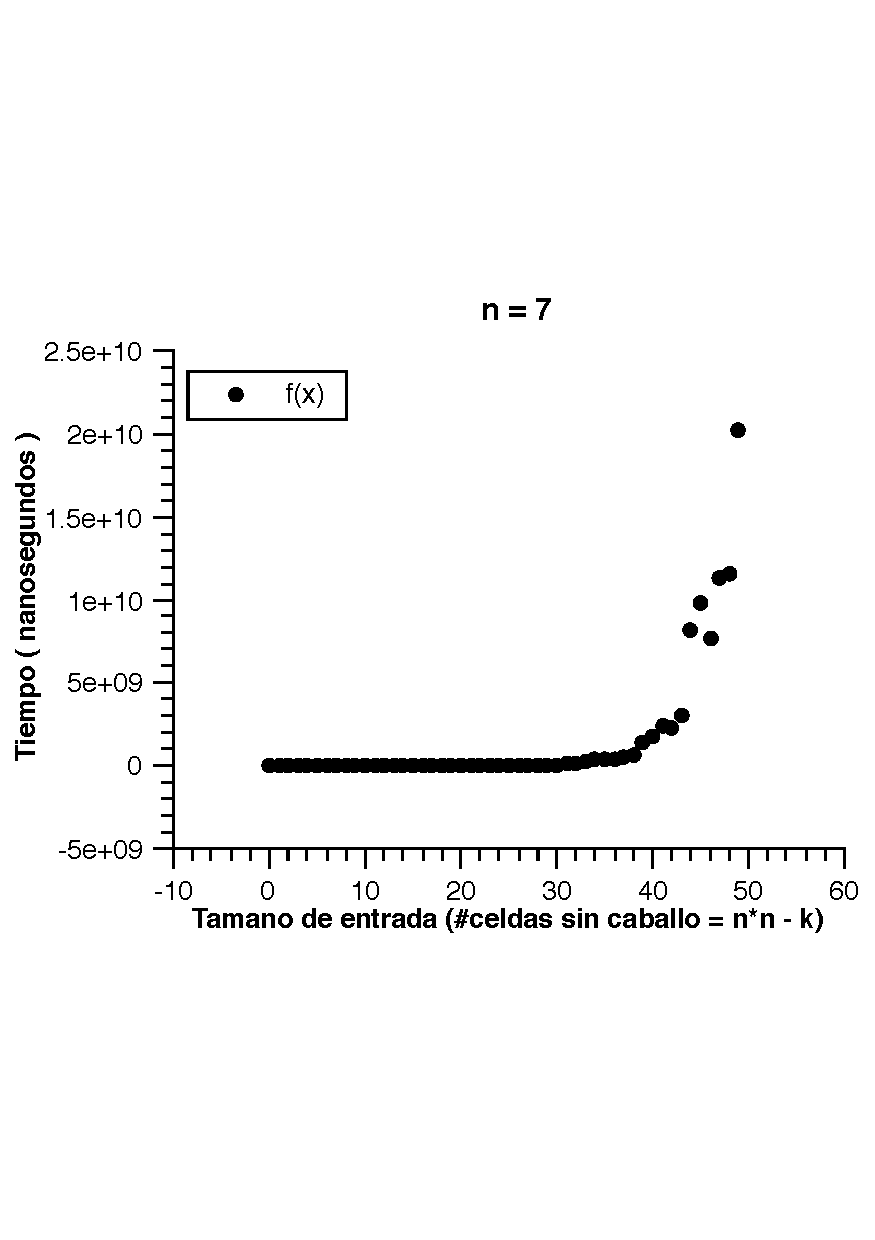
\includegraphics[width=\textwidth]{imagenes/grafico3-n-7-norm.pdf}
                \caption{Tiempos sin procesar}
        \end{subfigure}%
        ~ %add desired spacing between images, e. g. ~, \quad, \qquad, \hfill etc.
          %(or a blank line to force the subfigure onto a new line)
        \begin{subfigure}[b]{0.5\textwidth}
                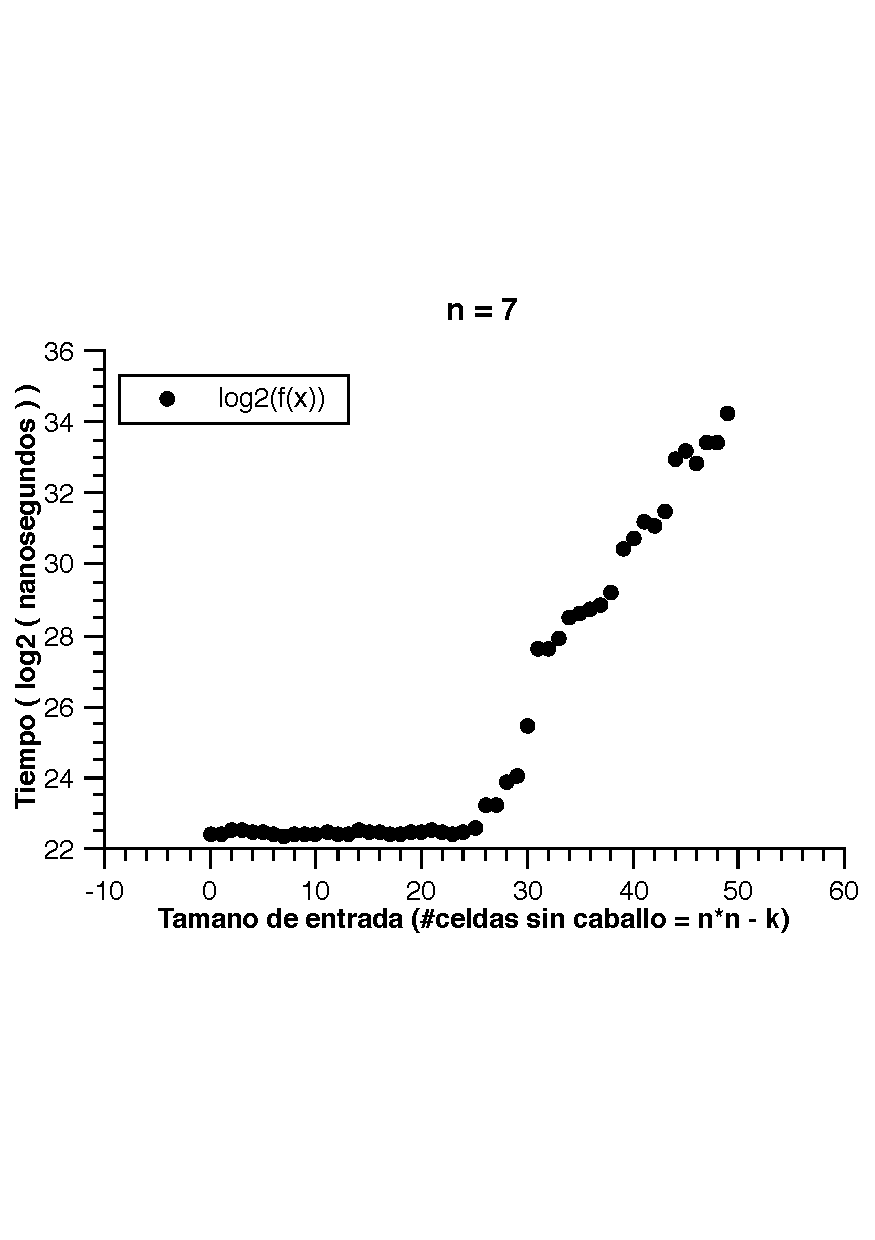
\includegraphics[width=\textwidth]{imagenes/grafico3-n-7-log.pdf}
                \caption{Logaritmo a la figura (a)}
        \end{subfigure}
        
        \begin{subfigure}[b]{0.5\textwidth}
                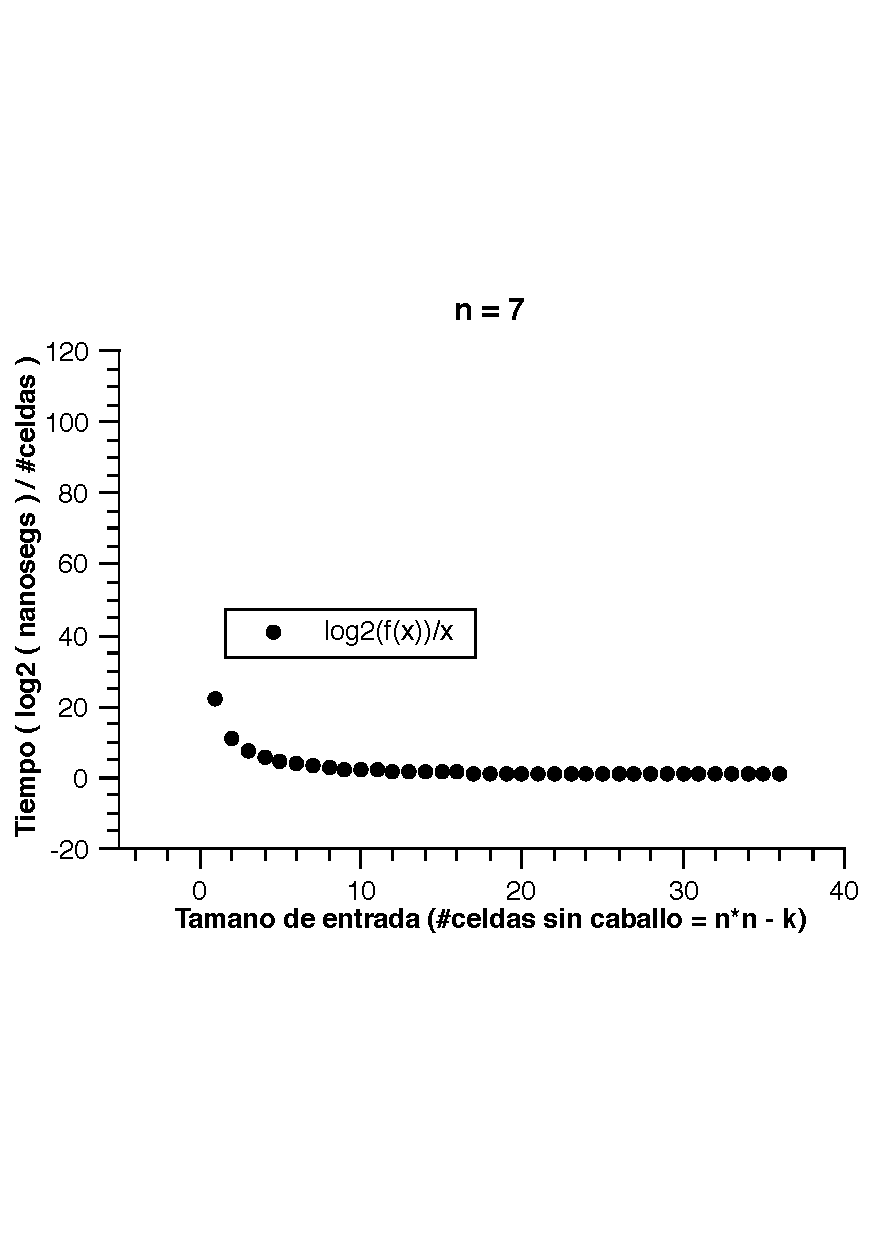
\includegraphics[width=\textwidth]{imagenes/grafico3-n-7-div-log.pdf}
                \caption{Dividiendo por x la figura (b)}
        \end{subfigure}
        \caption{Gráficos para $n=7$ sin podas G ni S}
\end{figure}

Con sus respectivas tablas en el Anexo \ref{sec:tablas-ej3}. \textit{Nota: se quitaron las podas G y S para facilitar el análisis del gráfico.}

Como podemos ver de los gráficos 1, 2 y 3 y sus respectivas tablas, al aplicarles logaritmo y dividirlos por x, todos tienden a un número constante entre cero y uno (para más detalles, se puede ver la tabla de valores en el anexo). Entonces nuestro algoritmo tendría complejidad $\mathcal{O}(c*2^{n^2 - k})$, donde $c$ es la constante a la cual converge el gráfico. Por lo tanto concluimos que los gráficos se condicen con nuestra predicción de complejidad.

\subsubsection{Experimentación con instancias particulares}

La experimentación con instancias particulares se realizó dejando el $k$ fijo en cero y variando el $n$ de 1 a 8:

\begin{figure}[H]
        \centering
        \begin{subfigure}[b]{0.5\textwidth}
                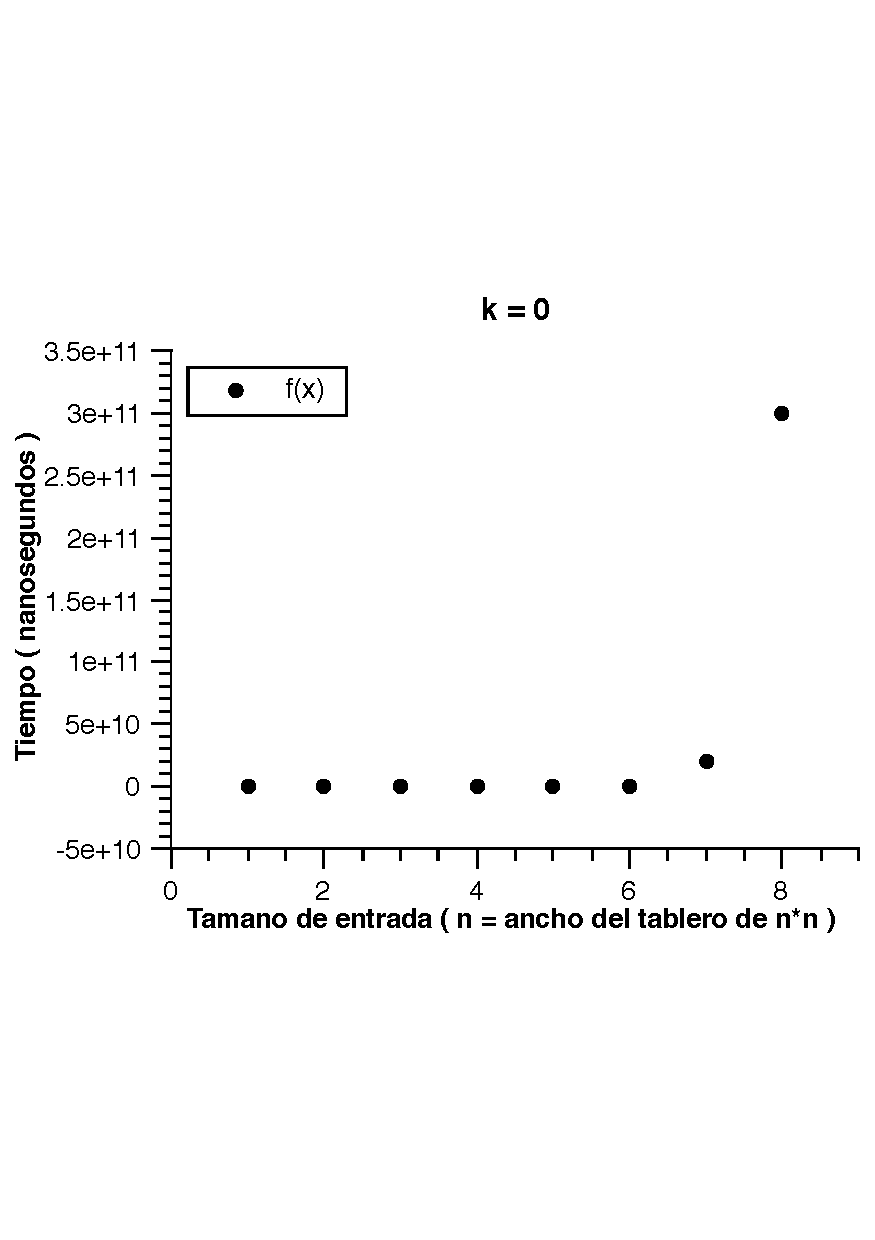
\includegraphics[width=\textwidth]{imagenes/grafico3-k-0-norm.pdf}
                \caption{Tiempos sin procesar}
        \end{subfigure}%
        ~ %add desired spacing between images, e. g. ~, \quad, \qquad, \hfill etc.
          %(or a blank line to force the subfigure onto a new line)
        \begin{subfigure}[b]{0.5\textwidth}
                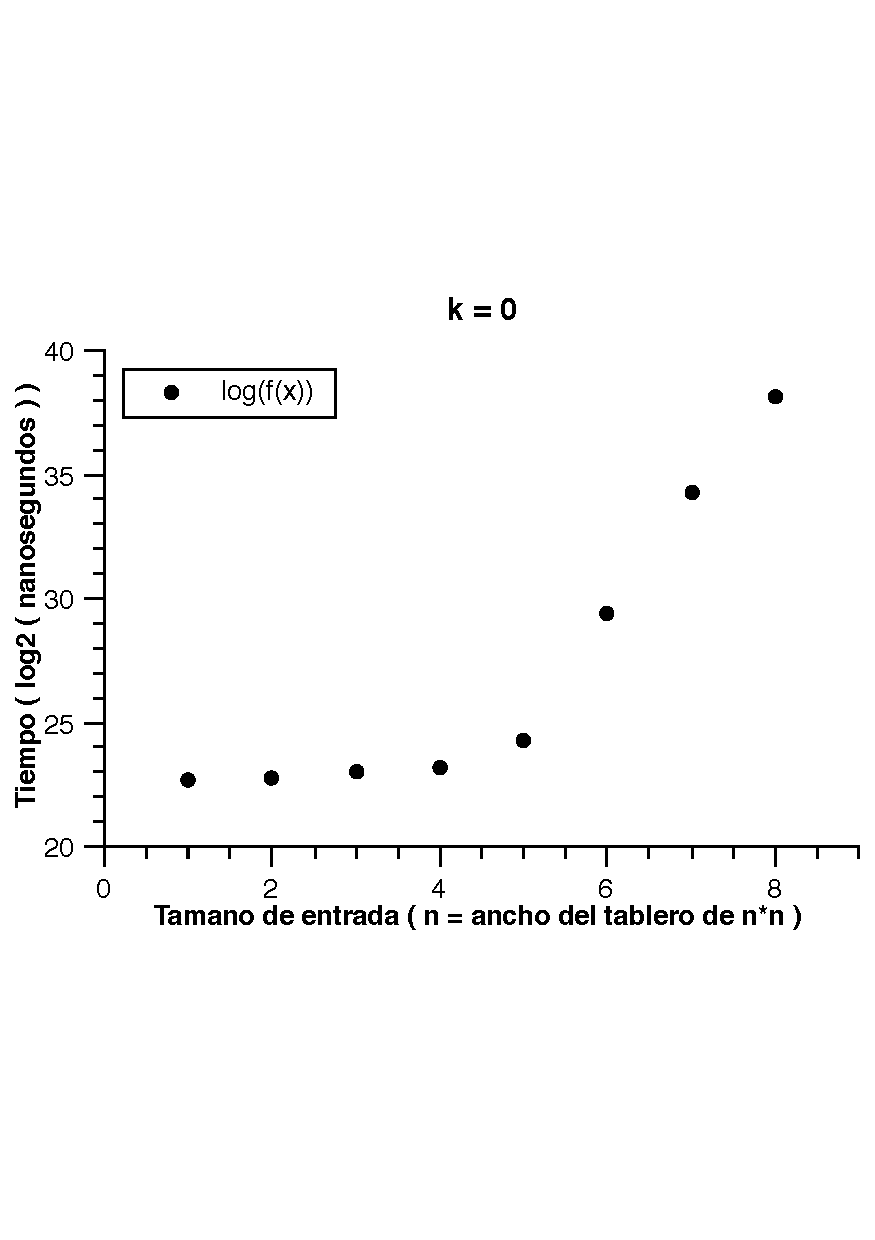
\includegraphics[width=\textwidth]{imagenes/grafico3-k-0-log.pdf}
                \caption{Logaritmo a la figura (a)}
        \end{subfigure}
        
        \begin{subfigure}[b]{0.5\textwidth}
                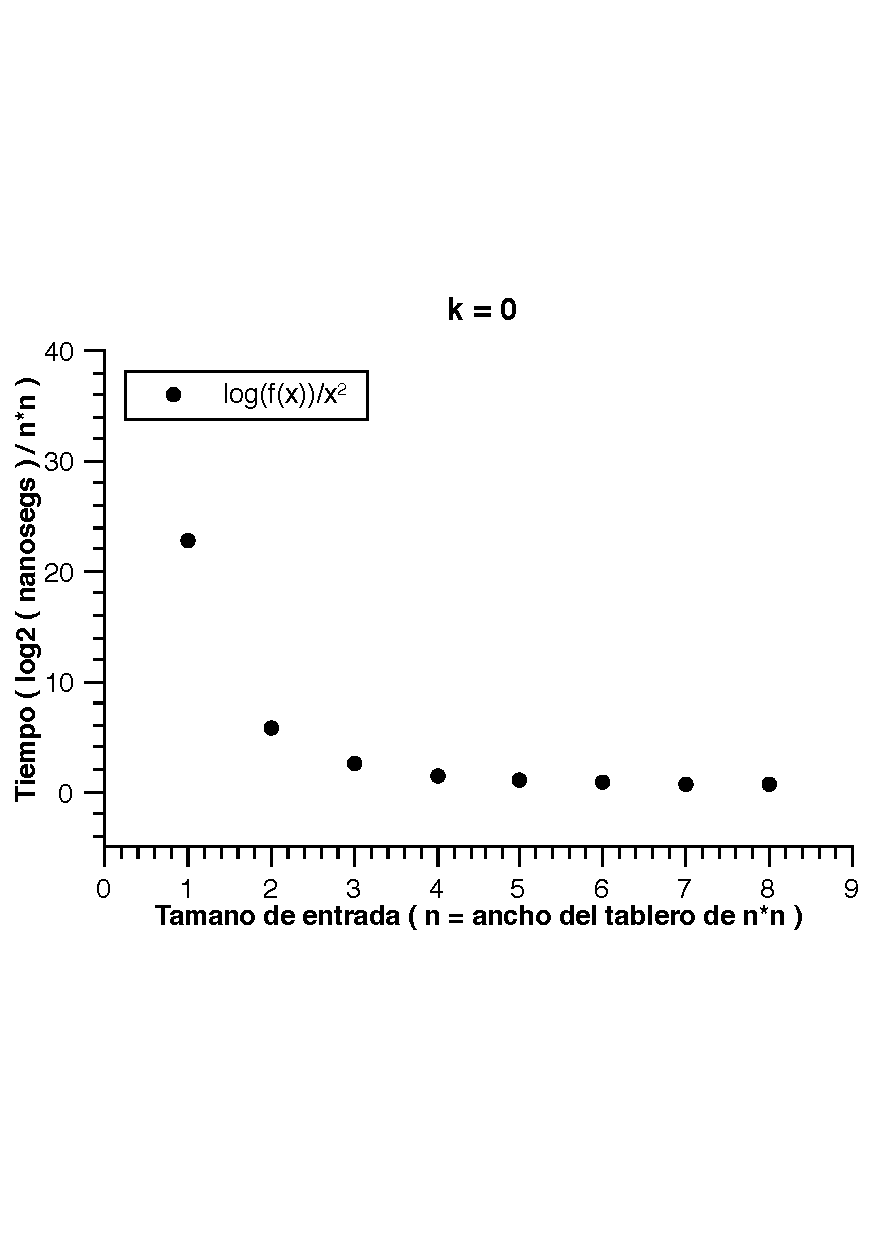
\includegraphics[width=\textwidth]{imagenes/grafico3-k-0-div-log.pdf}
                \caption{Dividiendo por x la figura (b)}
        \end{subfigure}
        \caption{Gráficos para $k=0$}
\end{figure}

Y su tabla también puede encontrarse en el Anexo \ref{sec:tablas-ej3}.

Para este experimento se utilizaron todas las podas detalladas anteriormente.
Se deprenden entonces los mismos resultados observados en los gráficos y tablas anteriores (el razonamiento es identico).

\subsubsection{Experimentación sin Podas}

Por último, se realizaron experimentaciones para comparar las mejoras aportadas por las podas:

\begin{figure}[H]
        \centering
        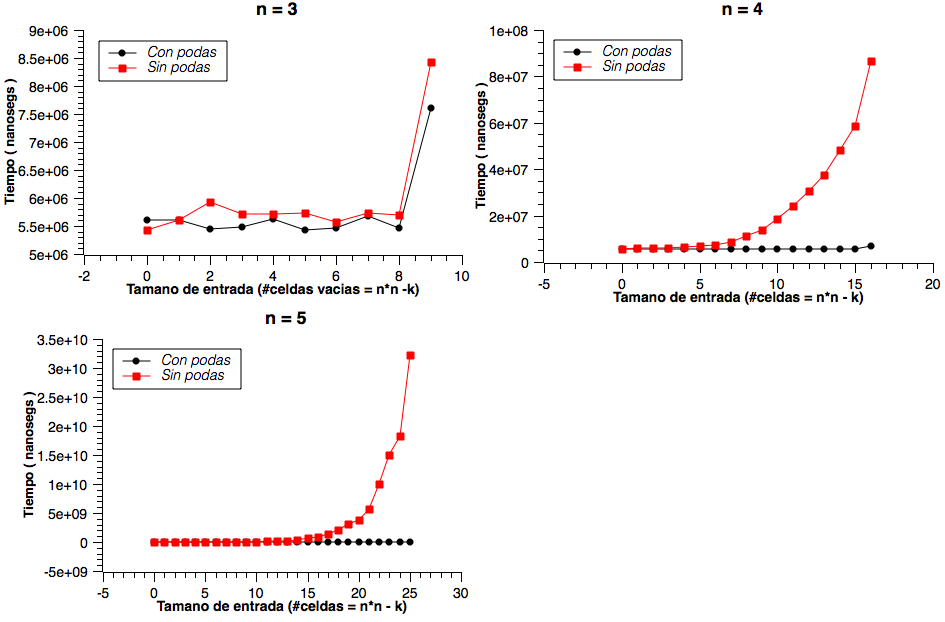
\includegraphics[width=\textwidth]{imagenes/grafico3-cmp-podas.png}
        \caption{Gráficos para $n=3,\ 4\ y\ 5$ comparando con podas vs. sin podas}
\end{figure}

\textit{Nota: el grafico sin podas sigue teniendo las podas B y C, ya que estás son las que hacen que el algoritmo devuelva soluciones correctas y no incorrectas.}

Y su tabla también puede hallarse en el Anexo  \ref{sec:tablas-ej3}.
